% Created 2024-02-11 Sun 20:23
% Intended LaTeX compiler: pdflatex
\documentclass[presentation]{beamer}
\usepackage[utf8]{inputenc}
\usepackage[T1]{fontenc}
\usepackage{graphicx}
\usepackage{longtable}
\usepackage{wrapfig}
\usepackage{rotating}
\usepackage[normalem]{ulem}
\usepackage{amsmath}
\usepackage{amssymb}
\usepackage{capt-of}
\usepackage{hyperref}
\mode<beamer>{\usetheme{Madrid}}
\definecolor{SUred}{rgb}{0.59375, 0, 0.17969} % SU red (primary)
\definecolor{SUblue}{rgb}{0, 0.17578, 0.38281} % SU blue (secondary)
\setbeamercolor{palette primary}{bg=SUred,fg=white}
\setbeamercolor{palette secondary}{bg=SUblue,fg=white}
\setbeamercolor{palette tertiary}{bg=SUblue,fg=white}
\setbeamercolor{palette quaternary}{bg=SUblue,fg=white}
\setbeamercolor{structure}{fg=SUblue} % itemize, enumerate, etc
\setbeamercolor{section in toc}{fg=SUblue} % TOC sections
% Override palette coloring with secondary
\setbeamercolor{subsection in head/foot}{bg=SUblue,fg=white}
\setbeamercolor{date in head/foot}{bg=SUblue,fg=white}
\institute[SU]{Shenandoah University}
\titlegraphic{\includegraphics[width=0.5\textwidth]{\string~/Documents/suLogo/suLogo.pdf}}
\newcommand{\R}{\mathbb{R}}
\usepackage{tikz}
\usepackage{pgfplots}
\usetheme{default}
\author{Chase Mathison\thanks{cmathiso@su.edu}}
\date{12 February 2024}
\title{Applied Right Triangle Trigonometry}
\hypersetup{
 pdfauthor={Chase Mathison},
 pdftitle={Applied Right Triangle Trigonometry},
 pdfkeywords={},
 pdfsubject={},
 pdfcreator={Emacs 29.1 (Org mode 9.6.7)}, 
 pdflang={English}}
\begin{document}

\maketitle

\section{Announcements}
\label{sec:org6eab4de}
\begin{frame}[label={sec:orgb0c187a}]{Announcements}
\begin{enumerate}
\item Homework in MyOpenMath
\item Office hours: M - F, 10am - 11am
\end{enumerate}
\end{frame}

\section{Lecture}
\label{sec:org9dc4a67}
\begin{frame}[label={sec:org829141a}]{Inclinometer Construction}
So how do we even measure this angle of elevation thing?

(One) Answer: An inclinometer!

You're going to make your own inclinometer now and we're going to go
out and measure some angles and see if we can find the height of some structures on campus.
\end{frame}

\begin{frame}[label={sec:org972b83c}]{Demonstration}
\end{frame}

\begin{frame}[label={sec:orgdf4403c}]{Applied Problems}
You want to measure the distance across a river.  To do this, you stand at the point \(A\)
in the picture below and measure the distance to point \(B\), and the angle made between
the lines \(AC\) and \(AB\).  What is the distance across the river?
\begin{center}
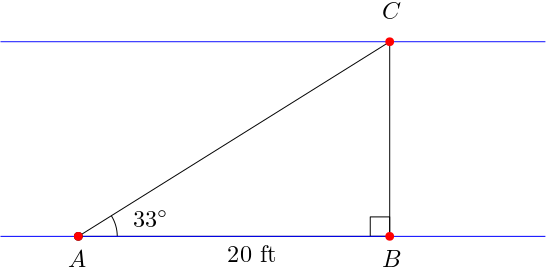
\includegraphics[width=0.5\textwidth]{./riverQ.png}
\end{center}
\end{frame}


\begin{frame}[label={sec:orga467375}]{Applied Problems}
\end{frame}

\begin{frame}[label={sec:org5aae2bf}]{Applied Problems}
The ancient greeks were able to measure the radius of the earth pretty accurately
using trigonometry.  Let's see how they did this.
(We'll need: Syrene -> Alexandria: 5000 stadia (or about 800 km).  Length of shadow about .1228 m)

\vspace{10in}
\end{frame}
\end{document}